\def \MOISEp {$\mathcal{M}OISE^+$} 
\def \MOISEpBf {$\mathbf{\mathcal{M}OISE^+}$} 

\chapter{Background}
\label{ch:background}

This chapter will explain the theoretical foundation for understanding this work, from the basics of multi-agent systems and modeling these systems to different control architectures used in robotics.

\section{Multi-agents systems}



\section{\MOISEpBf}

\MOISEp \cite{MOISEp} is a framework for modeling MAS developed by researchers from the University of São Paulo together with researchers from the Ecole Nationale Supérieure des Mines de Saint-Etienne, which extends its predecessor, called MOISE (Model of Organization for multI-agent SystEms) \cite{Moise}. Therefore, to better understand \MOISEp it is first necessary to comprehend the basics concepts of the MOISE model.

MOISE is a framework for designing and developing complex and dynamic organizations for multi-agent systems using an organization-centric point of view. The model provides a structured way of defining an organization so that all the agents work together in a coordinated and efficient manner, this structure is obtained by linking the roles that an agent can play to the plans that need to be executed for the organization to work as a whole. The model is divided into three levels:

\begin{itemize}
    \item \textit{Individual level}: The behavior that needs to be performed for a specific role.
    \item \textit{Social level}: The relationships between the roles.
    \item \textit{Collective level}: The aggregation of roles in large structures.
\end{itemize}

Nevertheless, certain limitations within MOISE required addressing to enhance the framework, such as the lack of the ability to explicitly define global plans for the system within the model. And it was for this reason that the model needed to be extended to the \MOISEp model \cite{MOISEp}. \MOISEp introduces three types of specifications that collectively define the framework: Structural Specification, Functional Specification, and Deontic Specification. These three specifications are essential for defining how the MAS organization works so it can reach its goal.

The \textbf{Structural Specification} delineates the organizational structure, defining the roles that the agents can play, their interrelationships, and group affiliations. This specification allows for the definition of hierarchical relationships, compatibility between roles, role authority, and other relevant characteristics. It also enables the specification of whether one role holds authority over another, the compatibility constraints between roles, and the number of agents that can be assigned to a particular role, among other structural details. An example of a \textbf{Structural Specification} from a MAS can be seen in Figure \ref{fig:moise_ss}.

\begin{figure}
    \centering
    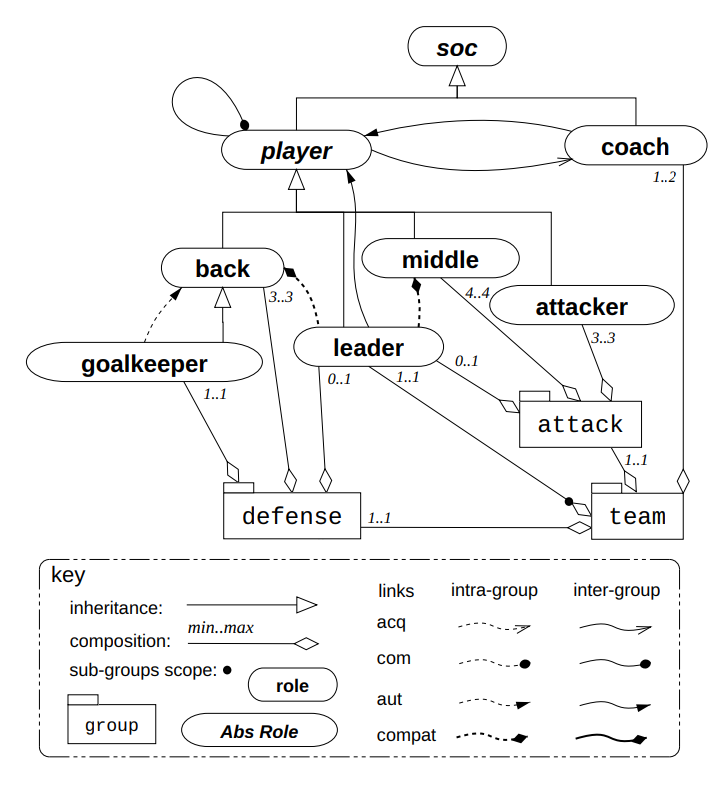
\includegraphics[width=0.75\linewidth]{images/MOISE - SS.png}
    \caption{Structural Specification of a soccer team. Taken from \cite{MOISEp}}
    \label{fig:moise_ss}
\end{figure}

From this example, it is possible to understand the different categories of links between the roles that exist. A link has two attributes, its type, presented in Table \ref{tab:types_of_links_in_moise}, and its scope, which can be intra-group or inter-group. An intra-group link is used to specify that an agent playing the link source role is linked to all agents playing the destination role within the group or any of its sub-groups. Meanwhile, an inter-group link connects despite the groups the agents it connects belongs to.

\def \sourceagent{$a_s$ }
\def \destagent{$a_d$ }

\begin{table}[!htbp]
    \begin{minipage}{\columnwidth}
        \centering
        \begin{tabular}{l l}
            \toprule
            Types         & Meaning                                                        \\
            \midrule
            Acquaintance  & \sourceagent is allowed to have a representation of \destagent \\
            Communication & \sourceagent is allowed to communicate with \destagent         \\
            Authority     & \sourceagent is allowed to have authority over \destagent      \\
            Compatibility & \sourceagent is also allowed to play the destination role      \\
            \bottomrule
        \end{tabular}
        \begin{center}
            \footnotesize 
            \emph{Note}: \sourceagent stands for the agent playing the source role of the link \\
            and \destagent stands for the agent playing the destination role. \\   
        \end{center}
    \end{minipage}
    \caption{Types of links between the roles in \MOISEp}
    \label{tab:types_of_links_in_moise}
\end{table}

Conversely, the \textbf{Functional Specification} is employed to define a way the goals of the organization can be achieved. It involves defining global plans, a structured way of combining goals, and utilizing a set of global goals to formulate missions. These missions serve as the foundation for the organization's social scheme, and agents within the organization can commit to missions in accordance with the rules defined in the social scheme of how many agents can commit to a specified mission. An example of a social scheme is illustrated in Figure \ref{fig:moise_fs}.

Lastly, the \textbf{Deontic Specification} establishes the relationship between the Structural and Functional Specifications by specifying the permissions and obligations associated with each role in relation to a mission. 

\begin{figure}[!h]
    \centering
    \begin{subfigure}{.44\linewidth}
        \centering
        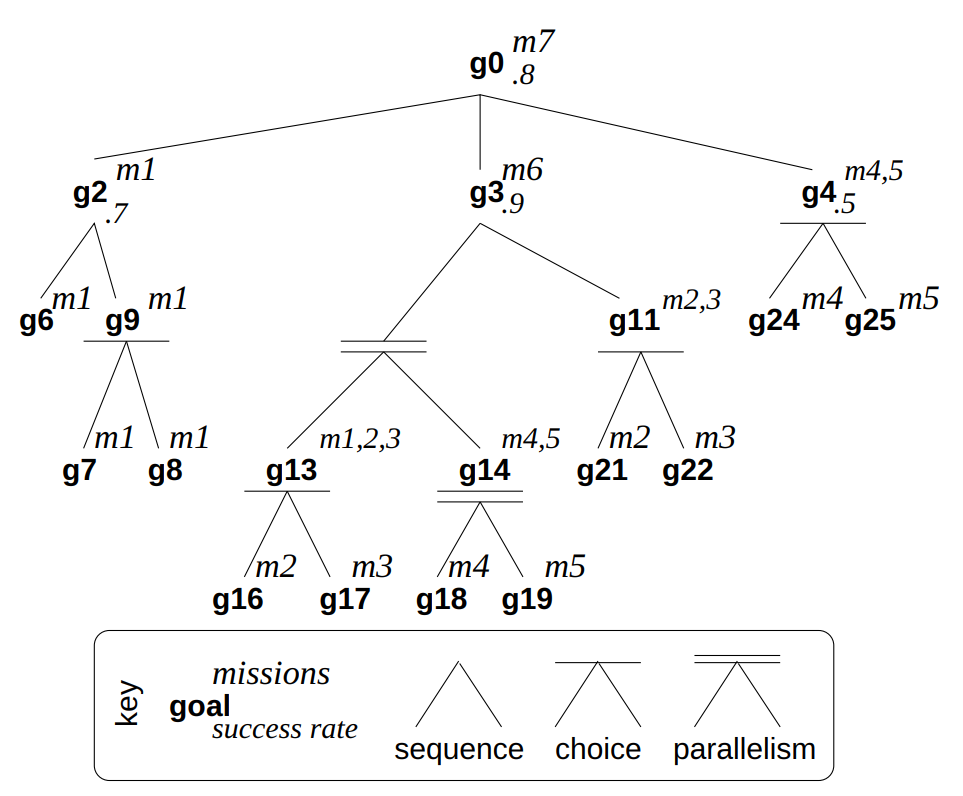
\includegraphics[width=\linewidth]{images/Moise - Social Scheme.png}
    \end{subfigure}
    \hfill
    \begin{subfigure}{.55\linewidth}
        \centering
        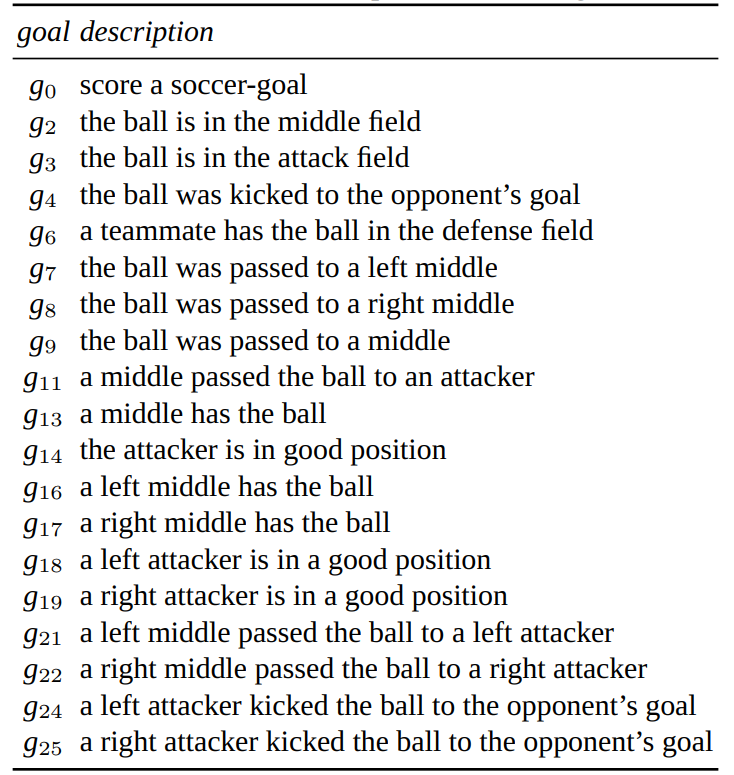
\includegraphics[width=0.8\linewidth]{images/Moise - Goals Descriptions.png}
    \end{subfigure}
    \caption{Example of Social Scheme to score a soccer goal. Taken from \cite{MOISEp}}
    \label{fig:moise_fs}
\end{figure}

\section{Control Architectures}

a

\section{Finite State Machines}

\section{Hierarchical State Machines}

\section{Behavior Trees}

% https://www.overleaf.com/learn/latex/Algorithms

% arrumar ref na implementacao sobre reactive

% \linkhttps{https://en.wikipedia.org/wiki/Behavior_tree_(artificial_intelligence,_robotics_and_control)}
% https://www.overleaf.com/learn/latex/TikZ_package
% https://forum.thunderatz.org/t/arquiteturas-de-controle/3640
% https://www.behaviortree.dev/docs/learn-the-basics/BT_basics

\subsection{Types of Nodes}

\subsubsection{Root Node} 

\subsubsection{Control Nodes} 
\label{subsubsec:control_nodes}

\subsubsection{Action Nodes}

\subsubsection{Condition Nodes}

\subsubsection{Decorator Nodes}

\subsubsection{Subtree Nodes}

\subsection{Reactivity}

\section{BT vs other Control Architectures}

\section{Blackboard}

\cite{BlackboardDesignPattern}
